%%
%%
%%      SECTION: SENSITIVITY
%%

%% \begin{figure}[htpb]
%% \begin{center}
%% %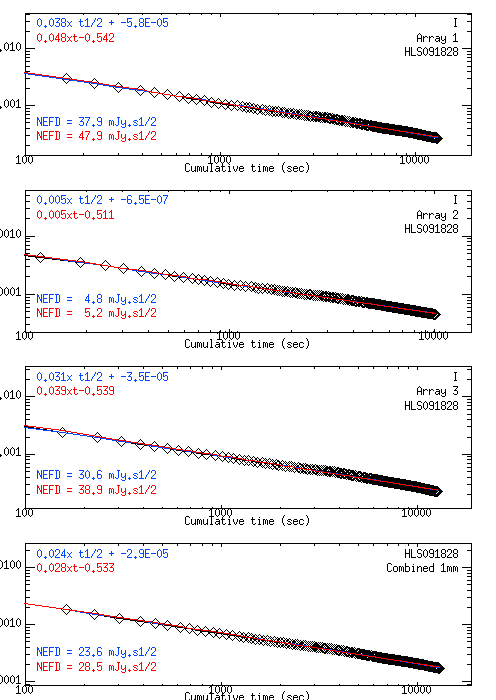
\includegraphics[clip, angle=0, scale =
%% %  0.5]{Figures/NEFD_HLS091828_20170226s415_FXDC0C1_GaussPhot.png}
%% %\includegraphics[clip, angle=0, scale = 0.5]{Figures/nefd_mpfit_HLS091828.eps}
%% \includegraphics[clip, angle=0, scale = 0.4]{Figures/HLS_fit.eps}
%% \includegraphics[clip, angle=0, scale = 0.4]{Figures/HLS_residuals.eps}
%% \caption{Sensitivity on \hls\ vs time of integration. Two power laws are fit:
%%   one with fixed slope $t^{1/2}$ that provides the estimate of the NEFD, one
%%   with a free slope $t^\beta$ to monitor the departure of noise integration from
%%   the canonical $t^{1/2}$. These data come from the integration on \hls\ during
%%   Run9. The difference between the 1 and 2~mm integration time comes from the
%%   density of KIDs in the FOV.}
%% \label{fig:nefd_vs_t}
%% \end{center}
%% \end{figure}

%% {\bf The specs/goals ``NEFD on X \% of pixels'' should be understood as : we have
%% XX\% valid pixels, and with these pixels, we have an NEFD of YY. We should not
%% discard some fraction of our pixels and estimate an NEFD on this subset.}\\

\section{Methodology {\color{blue} Nico}}

The MoU defines the NEFD:  \emph{The Noise Equivalent Flux Density (NEFD)
  is the $1\,\sigma$ sensitivity in one second of effective on-source telescope
  integration time after the absolute calibration has been performed (i.e. after
  beam efficiency and opacity corrections). It is appropriate for 2 mm of
  precipitable water vapor (pwv) content in the atmosphere and 60 degrees
  elevation source. It refers to the inverse variance of the noise on the flux
  measurement of a point-source, averaged over the valid receiver pixels}.

IRAM has its own time estimator for astronomers that will compute the ``effective NEFD'',
provided we give the ``detector NEFD'' and a fraction of valid KIDs $\eta$. To
derive the detector NEFD, we must clearly defined the ``detector time of
integration'' and relate it to the ``time of observation'' which is the time
actually spent by an astronomer at the observing desk. Going from the intuitive
understanding of the time of integration to its actual value is not as trivial
as it seems because of the dependence on the scanning strategy and the
distribution of valid KIDs accross the FOV. We here propose three definitions
with their own merits.

\subsection{Estimating the time of integration}

\subsubsection{Time of integration from the density of samples}

Let's take a map of resolution $r$ (arcsec) and consider the map pixel that is
centered on the position where we estimate the flux uncertainty
$\sigma_\phi$. The number of hits in this pixel $N_h(r)$ allows us to define a
time of integration on this pixel via the sampling frequency $\nu$

\begin{equation}
t_{pix} = N_h(r)/\nu
\end{equation}

To estimate how much wall clock time was necessary to the entire matrix to
produce this density of samples, we need to account for how many KIDs, on
average, contribute to $N_h(r)$ at the same time, that is to say the average
number of KIDs per map pixel. Indeed, if the pixel is large enough to contain
$n$ KIDs at each time, the number of samples in this pixel will be $n$ times
larger for the same time of observation. The same is true if we combine A1 and
A3 for instance. We therefore note $S$ the surface of the FOV, $g$ the distance
between adjacent KIDs and note that $S = N_{pix} \times r^2 = N_{kids} \times
g^2$. The number of KIDs per pixel of $r$\,arcsec resolution is thus $r^2/g^2$,
so the actual observation time reads

\begin{equation}
t_{det} = t_{pix}\frac{g^2}{r^2} = \frac{N_h(r)}{\nu}\frac{g^2}{r^2}
\end{equation}

For the combination of arrays 1 and 3, the number of KIDs per pixel is the sum
of the two contributions that impact the number of KIDs per pixel:

\begin{equation}
t_{det}^{1mm} = \frac{1}{2}\frac{N^{1mm}_h(r)}{\nu}\frac{g^2}{r^2}
\end{equation}

So finally, if $\sigma$ is the uncertainty on the flux estimate, the detector NEFD reads

\begin{equation}
NEFD_{det} = \sigma_\phi\sqrt{t_{det}}
\label{eq:nefd_t_int}
\end{equation}

To relate it to the effective ``observer'' NEFD, we must account for the
fraction of valid pixels actually used to derive the map. Indeed, the
integration time per pixel goes like $\eta$ for the same observation, thus:

\begin{equation}
NEFD_{det}^{eff} = \sigma_\phi\sqrt{t_{det}/\eta}
\end{equation}

which in turn translates into a time requirement to reach the same level of integration:

\begin{equation}
t_{det}^{req} = \left(\frac{NEFD_{det}}{\sigma_\phi}\right)^2\frac{1}{\eta}
\label{eq:t_astro}
\end{equation}

\subsubsection{Time of integration from the matrix footprint}

One can also think of the ``time spent on the source'', for a full matrix
(ie. all valid KIDs), as the time when the source is inside the circular
footprint of the matrix. During a scan, it's easy to count how much time the
source is at a distance from the FOV center that is smaller than the FOV
radius. This time, $t_{geom}$ is a direct estimate of the time ``at the desk'',
so it enters the definition of effective NEFD, not the detector NEFD, hence:

\begin{equation}
NEFD^{eff}_{geom} = \sigma_\phi \sqrt{t_{geom}}
\end{equation}

Fig.~\ref{fig:integration_time} compares $\eta t_{geom}$ to $t_{det}$ and shows
the good agreement between the two.


\subsubsection{Time of integration from the flux estimator}

The estimation of the flux of a point source, and its associated uncertainty is
done by fitting the amplitude of a gaussian profile of fixed FWHM. In the case
of white noise, the flux estimator reads

\begin{equation}
\hat{\phi} = \frac{1}{\sum_p g_p^2}\sum_p g_p m_p\,,
\label{eq:phi_def}
\end{equation}

and its variance is

\begin{equation}
\sigma_\phi^2 = \left(\frac{1}{\sum_p g_p^2}\right)^2\sum_p g_p^2\sigma_p^2\,.
\label{eq:sigma_phi_def}
\end{equation}

In the case of white noise and considering the equivalent of the
uniform full matrix of the NEFD definition: $\sigma_p = \sigma_1/\sqrt{N_p}$,
where $\sigma_1$ is the standard deviation of 1 sample and $N_p$ is the number of
hits in pixel $p$. Accounting for the sampling frequency, it reads

\begin{eqnarray}
\sigma_\phi^2 &=& \frac{\sigma_1}{\nu}\left(\frac{1}{\sum_p g_p^2}\right)^2\sum_p \frac{g_p^2}{t_p}\,, \nonumber\\
&=&\frac{\sigma_1}{\nu}\frac{1}{t_{beam}}\,
\label{eq:sigma_phi_def_2}
\end{eqnarray}

where $t_{beam}$ is homogeneous to a time and is such that $\sigma_\phi$ goes
like $1/\sqrt{t_{beam}}$.

\begin{figure}
\begin{center}
\includegraphics[clip, angle=0, scale =0.8]{Figures/Pluto_time_of_integration.eps}
\caption[Time of integration]{Comparison between three estimators of the time of integration on the
  source during Pluto's observation (Run9). To a few percent, the 3 estimators
  give compatible estimations.}
\label{fig:time_comparison}
\end{center}
\end{figure}


%% Note: there is no way to be perfectly precise on the estimation of these
%% parameters, in all circumstances, on the edges of any matrix, for potential
%% areas covered by A1 and not A3 (or just less). Like in any case, we must live
%% with this, focus on the main area of each scan and forget about edge effects.

%\section{History and confusions}

%In the past few days, we have re-examined these definitions, and several
%mistakes were made:

%\begin{itemize}
%\item at some point, the {\tt nk\_map\_photometry.pro} that is supposed to give
%  the correct ``time'', rather than giving $t_{int}$ as defined in
%  Eq.~(\ref{eq:t_int}) was giving $\eta t_{int}$.
%\item When questioning this relation, we confused $t_{int}$ and $t_{obs} = t_{int}/\eta$. While
%  the dependence on the grid step and the map resolution was accounted for in
%  average, it was not the correct time to consider to compute the NEFD as defined in
%  the MoU (a.k.a detector NEFD, letting $\eta$ as another parameter in IRAM's
%  time estimator).
%\item In the end, the final NEFD we must give to IRAM are those that we
%  published but increased by a factor $1/\sqrt{\eta}$.
%\end{itemize}


\subsection{NEFD estimation methods}

To perform consistency and robustness test, we have developped three methods for
the NEFD estimation. Namely, Methods 1 and 2 relie on deep integration on faint
source: while Method 1 estimates the NEFD from a fit of the evolution of the
flux density uncertainties with the integration time, Method 2 resorts to
combining the scans in order to annulate the signal and obtain noise
estimates. Detailed methodology and results are discussed in
Sect.~\ref{NEFD_deep}. Method 3 consists in i) estimating an NEFD per
point-source scan by evaluating the flux noise from map pixels far from the
source and ii) studying the NEFD distribution as a function of the atmospheric
attenuation to report the NEFD estimate for the appropiate observing
conditions. Method 3 results are presented in Sect.~\ref{NEFD_pipeline}.

